\section{Алгебра логики} \label{sec:boolean}

\defemph{Математика}~--- это общий язык для многих сфер деятельности человека, позволяющий формализовать объекты, которыми оперирует наш разум.
Однним из важнейших разделов математики считается \defemph{математическая логика},
так как именно она является фундаментом математических суждений, исследует природу математического доказательства в целом.
Поэтому не зря курс дискретного анализа начинается именно с \defemph{алгебры логики}~---
объекта математической логики, хоть и сравнительно простого, но важного и полезного.



\subsection{Булева алгебра}
\label{subsec:boolean:algebra}


Алгебра логики изучает логические операции над высказываниями.
При этом в простейшем случае считается, что высказывания могут быть только истинными (обозначается~<<$ 1 $>>) или ложными (обозначается~<<$ 0 $>>);
%такие высказывания являются \defemph{булевозначными}.

\begin{definition}
    Переменные, принимающие значения только $ 0 $ или $ 1 $, называются \defemph{булевыми переменными}.
    Аналогично, функции от булевых переменных, принимающие только значения $ 0 $ или $ 1 $~--- \defemph{булевы функции}, или \defemph{логические операции}, \defemph{связки}.
    \defemph{Высказываниям} ставится в соответствие либо булева переменная с фиксированным значением, либо значение булевой функции на фиксированных аргументах.
\end{definition}

Примеры логических операций:
<<НЕ>> (обозначается~<<$ \neg $>>),
<<И>> (обозначается~<<$ \wedge $>>),
<<ИЛИ>> (обозначается <<$ \vee $>>),
исключающее <<ИЛИ>> (обозначается <<$ \oplus $>>),
импликация (обозначается <<$ \rightarrow $>>),
эквивалентность (обозначается <<$ \leftrightarrow $>>).

Заметим, что как и любые другие функции с конечной областью определения, булевы функции можно задать таблицей, просто перечислив их значения на всех возможных значениях аргументов.
Данные таблицы называются \defemph{таблицами истинности}.

\begin{table}[ht!]
    \center
    \begin{tabular}{|c|c|c|c|c|c|c|c|}
         \hline
         $ A $  &  $ B $  &  $ \neg A $  &  $ A \wedge B $  &  $ A \vee B $  &  $ A \oplus B $  &  $ A \rightarrow B $  &  $ A \leftrightarrow B $ \\
         \hline
         \hline
         $ 0 $  &  $ 0 $  &  $ 1 $       &  $ 0 $           &  $ 0 $         &  $ 0 $           &  $ 1 $                &  $ 1 $                   \\
         $ 0 $  &  $ 1 $  &  $ 1 $       &  $ 0 $           &  $ 1 $         &  $ 1 $           &  $ 1 $                &  $ 0 $                   \\
         $ 1 $  &  $ 0 $  &  $ 0 $       &  $ 0 $           &  $ 1 $         &  $ 1 $           &  $ 0 $                &  $ 0 $                   \\
         $ 1 $  &  $ 1 $  &  $ 0 $       &  $ 1 $           &  $ 1 $         &  $ 0 $           &  $ 1 $                &  $ 1 $                   \\
         \hline
    \end{tabular}
    \caption{задание логических связок таблицами истинности}
    \label{tab:boolean:truth_tables}
\end{table}

%\begin{Exercise}[counter=SecExercise, title=(КЗ №1)]
%    \noindent
%    Для какого слова \textbf{ложно} высказывание <<Первая буква слова гласная $ \rightarrow $ (Вторая буква слова гласная $ \vee $ Последняя буква слова гласная)>>?
%    \begin{enumerate}[label=\arabic*)]
%        \item жара;
%        \inlineitem орда;
%        \inlineitem огород;
%        \inlineitem парад;
%    \end{enumerate}
%\end{Exercise}
%
%\begin{Answer}
%    \noindent
%    Подставляя слова в элементарные высказывания, получаем
%    \begin{enumerate}
%        \item $ 0 \rightarrow (1 \vee 1) = 1 $;
%        \item $ 1 \rightarrow (0 \vee 1) = 1 $;
%        \item $ 1 \rightarrow (0 \vee 0) = 0 $;
%        \item $ 0 \rightarrow (1 \vee 0) = 1 $;
%    \end{enumerate}
%    Можно было сразу отсеять первый и четвёртый варинат по ложной посылке, а ответ найти по ложному следствию.
%\end{Answer}

%\shipoutAnswer

Запись таблицы истинности можно сократить, если изначально условиться, в каком порядке перечисляются возможные значения аргументов, и оставить только столбец значений функции;
этот столбец тогда будет являться \defemph{булевым вектором} (\defemph{вектором значений}), задающим функцию.
Стандартный порядок перечисления значений аргументов таков, чтобы они образовывали двоичную запись номера строки (см. таблицу \ref{tab:boolean:truth_tables}).

\begin{example}
    Операция <<НЕ>> задаётся булевым вектором $ 10 $, а, например, импликация~--- $ 1101 $.
\end{example}

Булевы функции можно также задавать при помощи формул, <<собирая>> из других связок.
Вообще говоря, формула является деревом, задающим порядок применения составляющих формулу связок к аргументам и к значениям других связок.
Однако такой взгляд на вещи полностью эквивалентен стандартному написанию математических формул, если задать приоритет операций, или просто использовать скобки.
Приоритет изученных связок указан в таблице \ref{tab:boolean:full_info}, пример формулы и соответствующего ей дерева~--- на рис. \ref{fig:boolean:tree_example}.

\begin{table}[ht!]
    \center
    \begin{tabular}{|c|c|c|c|c|c|}
        \hline
        Связка               & Приоритет & \makecell{Краткое \\ название}     & Название        & Смысл                       \\
        \hline
        \hline
        $ \neg $             & $ 1 $     & <<НЕ>>                             & отрицание       & <<не $ A $>>                \\
        $ \wedge $           & $ 2 $     & <<И>>                              & конъюнкция      & <<$ A $ и $ B $>>           \\
        $ \vee $             & $ 3 $     & <<ИЛИ>>                            & дизъюнкиця      & <<$ A $ или $ B $>>         \\
        $ \oplus $           & $ 3 $     & \makecell{<<ИСКЛИЛИ>>, \\ <<XOR>>} & исключающее или & <<либо $ A $, либо $ B $>>  \\
        $ \rightarrow $      & $ 4 $     & --                                 & импликация      & <<если $ A $, то $ B $>>    \\
        $ \leftrightarrow $  & $ 5 $     & --                                 & эквивалентность & <<$ A $ равносильно $ B $>> \\
        \hline
    \end{tabular}
    \caption{информация о логических связках}
    \label{tab:boolean:full_info}
\end{table}


\begin{figure}[ht!]
    \center
    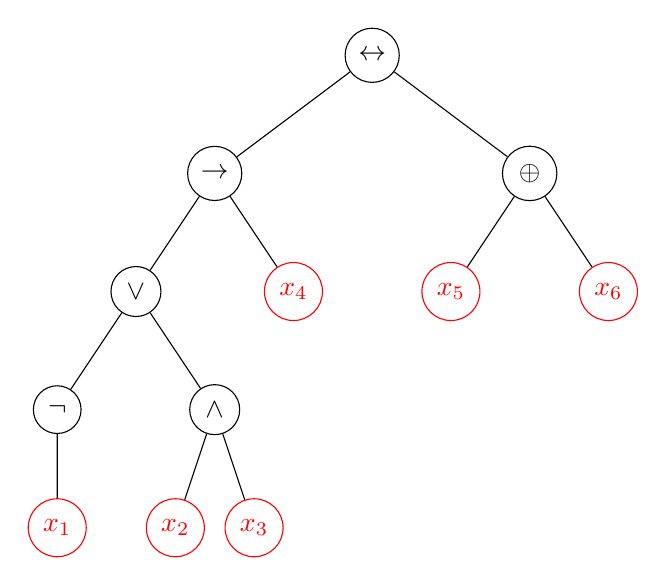
\begin{tikzpicture}[level distance=1.5cm,
        level 1/.style={sibling distance=4cm},
        level 2/.style={sibling distance=2cm},
        level 4/.style={sibling distance=1cm}
        %edge from parent/.style={draw, edge from parent path={(\tikzparentnode) -- (\tikzchildnode)}}
    ]
    \tikzstyle{every node}=[circle,draw]

    \node (Root) {$ \leftrightarrow $}
        child {
            node {$ \rightarrow $}
            child {
                node {$ \vee $}
                child {
                    node {$ \neg $}
                    child { node[red] { $x_1 $} }
                }
                child {
                    node {$ \wedge $ }
                    child { node[red] { $ x_2 $ } }
                    child { node[red] { $ x_3 $ } }
                }
            }
            child { node[red] {$ x_4 $} }
        }
        child {
            node {$ \oplus $}
            child { node[red] {$ x_5 $} }
            child { node[red] {$ x_6 $} }
        };

    \end{tikzpicture}
    \caption{дерево формулы $ \neg x_1 \vee x_2 \wedge x_3 \rightarrow x_4 \leftrightarrow x_5 \oplus x_6 $
    (или, что то же самое, $ (((\neg x_1) \vee (x_2 \wedge x_3)) \rightarrow x_4) \leftrightarrow (x_5 \oplus x_6) $)}
    \label{fig:boolean:tree_example}
\end{figure}

\FloatBarrier



\subsection{Логические законы}
\label{subsec:boolean:laws}



\defemph{Логический закон} (\defemph{тождество})~--- равенство двух булевых функций, заданных разными формулами.
Равенство булевых функций определяется так же, как и равенство любых других функций:
требуется равенство областей определений функций и равенство значений функций в любой точке области определения.
Равенство формул и области определения, очевидно, влечет равенство функций; обратное не верно.
Принято также считать, что если аргументы в формуле пронумерованы, то число аргументов равно максимальному индексу (<<нет пропусков>>).

\begin{example}
    \label{example:boolean:formulas}
    \begin{itemize}
        \item[] % КОСТЫЛЬ! :(
        \item С точки зрения правил школьной математики, функции $ \sqrt[3]{x} $ и $ (x)^{1/3} $ не равны.
        \item Формула, задающая функцию трёх аргументов: $ x_1 \wedge x_3 $.
        \item Две формулы, задающие одну и ту же функцию: $ x_1 \rightarrow x_2 $ и $ \neg x_1 \vee x_2 $.
        \item Равенство областей определения \textbf{существенно}: пусть
            \[
                f(A,B,C) = A \vee B, \quad g(A,B) = A \vee B
            \]
            Данные две функции заданы одной и той же формулой, но $ f \neq g $.
    \end{itemize}
\end{example}

В случае булевых функций определение равенства можно записать иначе, если воспользоваться понятием \defemph{тавтологии}.

\begin{definition}
    Функция $ g $ называется \defemph{тавтологией} $ \defarr $ она тождественна равна единице на всей области определения.
\end{definition}

\begin{remark}
    Для булевых функций $ f $ и $ g $ их равенство эквивалентно равенству областей определений и тавтологичности $ f \leftrightarrow g $.
\end{remark}


Пользуясь определением связок из таблицы \ref{tab:boolean:truth_tables}, можно доказать множество логических законов. %(тождеств).
Самые тривиальные законы~--- \textit{коммутативность} и \textit{ассоциативность} операций $ \wedge $, $ \vee $ и $ \oplus $:
\[
    x_1 \wedge x_2 = x_2 \wedge x_1, \qquad
    x_1 \vee x_2   = x_2 \vee x_1, \qquad
    x_1 \oplus x_2 = x_2 \oplus x_1
\]
\[
    x_1 \wedge (x_2 \wedge x_3) = (x_1 \wedge x_2) \wedge x_3, \qquad
    x_1 \vee (x_2 \vee x_3)     = (x_1 \vee x_2) \vee x_3, \qquad
    x_1 \oplus (x_2 \oplus x_3) = (x_1 \oplus x_2) \oplus x_3
\]
Также имеет смысл выписать некоторые \textit{дистрибутивные} законы:
\[
    x_1 \wedge (x_2 \vee x_3) = (x_1 \wedge x_2) \vee (x_1 \wedge x_3)
\]
\[
    x_1 \vee (x_2 \wedge x_3) = (x_1 \vee x_2) \wedge (x_1 \vee x_3)
\]
Другие полезные законы:
\begin{enumerate}[label=\arabic*)]
    \item $ x_1 \vee (x_1 \wedge x_2) = x_1; \quad x_1 \wedge (x_1 \vee x_2) = x_1 $ \hspace*{\fill} \textit{(законы поглощения)}
    \item $ \neg (x_1 \wedge x_2) = \neg x_1 \vee \neg x_2; \quad \neg (x_1 \vee x_2) = \neg x_1 \wedge \neg x_2 $ \hspace*{\fill} \textit{(законы де Моргана)}
    \item $ x_1 \rightarrow x_2 = \neg x_2 \rightarrow \neg x_1 $ \hspace*{\fill} \textit{(закон контрапозиции)}
    %\item $ (x_1 \rightarrow x_2) \vee x_3 = x_1 \rightarrow (x_2 \vee x_3) $ \hspace*{\fill} \textit{(внос в следствие)}
    \item $ x_1 \leftrightarrow x_2 = \neg (x_1 \oplus x_2) = (x_1 \rightarrow x_2) \wedge (x_2 \rightarrow x_1) $
    \item $ x_1 \to x_2 = \neg x_1 \vee x_2 $ \label{item:implication_disjunction}
\end{enumerate}
Остальные законы и свойства можно найти в конспекте лекций Александра Александровича.
Отдельно отметим, что из пункта \ref{item:implication_disjunction} следует,
что импликация дистрибутивна относительно конъюнкции:
\[
    x_1 \rightarrow (x_2 \wedge x_3) = \neg x_1 \vee (x_2 \wedge x_3) = (\neg x_1 \vee x_2) \wedge (\neg x_1 \vee x_3) = (x_1 \rightarrow x_2) \wedge (x_1 \rightarrow x_3)
\]

\begin{Exercise}[counter=SecExercise, label={ex:boolean:chain}]
    \noindent
    Докажите равенство функций
    \[
        (x_1 \rightarrow x_2) \wedge (x_2 \rightarrow x_3) \wedge \ldots \wedge (x_{k-1} \rightarrow x_k) \wedge (x_k \rightarrow x_1) =
        \left( \bigwedge_{i=1}^{k-1} (x_i \rightarrow x_{i+1}) \right) \wedge (x_k \rightarrow x_1)
    \]
    и
    %\[
    %    (x_1 \leftrightarrow x_2) \wedge (x_2 \leftrightarrow x_3) \wedge \ldots \wedge (x_{k-1} \leftrightarrow x_k) \wedge (x_k \leftrightarrow x_1) =
    %    \left( \bigwedge_{i=1}^{k-1} (x_i \leftrightarrow x_{i+1}) \right) \wedge (x_k \leftrightarrow x_1)
    %\]
    \[
        x_1 \leftrightarrow x_2 \leftrightarrow x_3 \leftrightarrow \ldots \leftrightarrow x_k
    \]
\end{Exercise}

\begin{Answer}
    \noindent
    % Несложно заметить, что если $ \forall i, j \; x_i = x_j $, то оба высказывания истинны.
    % Если же $ \exists i,j: \; x_i \neq x_j $, то второе высказывание ложно.
    % Но что насчёт первого?
    % Понятно, что раз $ \exists i,j: \; x_i \neq x_j $, то и $ \exists m: \; x_m = 1 \neq 0 = x_{m+1} $
    % (считаем, что $ x_{k+1} = x_1 $, то есть нумерация зациклена).
    % Но тогда и первое высказывание ложно.
    %% ВЕРСИЯ БЕЗ КВАНТОРОВ %%
    Несложно заметить, что если при любых $ i, j $ выполнено $ x_i = x_j $, то оба высказывания истинны.
    Если же существуют $ i,j $ такие, что $ x_i \neq x_j $, то второе высказывание ложно.
    Но что насчёт первого?
    Понятно, что раз существуют $ i,j $ такие, что $ x_i \neq x_j $, то и существует $ m $ такое, что $ x_m = 1 \neq 0 = x_{m+1} $
    (считаем, что $ x_{k+1} = x_1 $, то есть нумерация зациклена).
    Но тогда и первое высказывание ложно.
\end{Answer}



\subsection{Преобразование и упрощение формул}
\label{subsec:boolean:transformation}



Преобразование формул при помощи одних тождеств позволяют находить другие.
Так при помощи привёдённых в предыдущем разделе законов можно доказать следующее утверждение:
\begin{statement}[Закон вноса в посылку и следствие]
    \label{statement:boolean:disjunction_implication}
    Верны тождества
    \[
        (x_1 \rightarrow x_2) \vee x_3 = x_1 \rightarrow (x_2 \vee x_3) = (x_1 \vee x_3) \rightarrow (x_2 \vee x_3)
    \]
\end{statement}

\begin{proof}
    Первое равенство доказывается тривиально:
    \[
        (x_1 \rightarrow x_2) \vee x_3 = \neg x_1 \vee x_2 \vee x_3 = \neg x_1 \vee (x_2 \vee x_3) = x_1 \rightarrow (x_2 \vee x_3)
    \]
    Перейдём ко второму.
    Для этого распишем импликацию через дизъюнкцию и воспользуемся правилом де Моргана:
    \[
        (x_1 \vee x_3) \rightarrow (x_2 \vee x_3) =
        \neg (x_1 \vee x_3) \vee x_2 \vee x_3 =
        (\neg x_1 \wedge \neg x_3) \vee x_2 \vee x_3
    \]
    Воспользовавшись дистрибутивностью дизъюнкции относительно конъюнкции, получаем
    \begin{multline*}
        (\neg x_1 \wedge \neg x_3) \vee x_2 \vee x_3 =
        \left[ (\neg x_1 \vee x_3) \wedge (\neg x_3 \vee x_3) \right] \vee x_2 = \\ =
        \left[ (\neg x_1 \vee x_3) \wedge 1 \right] \vee x_2 =
        \neg x_1 \vee x_3 \vee x_2 =
        x_1 \rightarrow (x_2 \vee x_3)
    \end{multline*}
\end{proof}

%При помощи доказанного факта решим следующую задачу:
\begin{Exercise}[counter=SecExercise, label={ex:boolean:disjunction_distributivity_over_equivalence}]
    \noindent
    Докажите дистрибутивность дизъюнкции относительно эквивалентности:
    \[
        x \vee (y \leftrightarrow z) = (x \vee y) \leftrightarrow (x \vee z)
    \]
\end{Exercise}

\begin{Answer}
    \noindent
    Пойдём от конца, начиная цепочку эквивалентных преобразований от правой формулы.
    Перепишем эквивалентность через две импликации:
    \[
        (x \vee y) \leftrightarrow (x \vee z) = \left[ (x \vee y) \rightarrow (x \vee z) \right] \wedge \left[ (x \vee z) \rightarrow (x \vee y) \right]
    \]
    Вынесем дизъюнкцию из посылки и следствия (см. утверждение \ref{statement:boolean:disjunction_implication}):
    \[
        \left[ x \vee \left( y \rightarrow z \right) \right] \wedge \left[ x \vee \left( z \rightarrow y \right) \right]
    \]
    Воспользуемся дистрибутивностью дизъюнкции относительно конъюнкции и <<вынесем $ x $ за скобки>>:
    \[
        x \vee \left( \left[ y \rightarrow z \right] \wedge \left[ z \rightarrow y \right] \right)
    \]
    Наконец, собирая обратно операцию эквивалентности, получаем искомую формулу:
    \[
        x \vee (y \leftrightarrow z)
    \]
    Заметим, что из связи дизъюнкции и импликации (см. тождество \ref{item:implication_disjunction}) также имеем
    \[
        x \rightarrow (y \leftrightarrow z) = (x \rightarrow y) \leftrightarrow (x \rightarrow z)
    \]
\end{Answer}


В последнем пункте примера \ref{example:boolean:formulas} видно, что значение $ f $ не зависит от значения $ C $.
В этом случае говорится, что $ C $~--- \defemph{несущественная} или \defemph{фиктивная переменная}.

\begin{definition}
    $ x_i $ ~--- \defemph{фиктивная переменная} функции $ f(x_1, \ldots, x_k) $ $ \defarr $ $ f \big|_{x_i = 0} $ и $ f \big|_{x_i = 1} $ равны как функции,
    то есть
    \[
        \forall x_1, \ldots, x_{i-1}, x_{i+1}, \ldots x_k \quad f(x_1, \ldots, x_{i-1}, 0, x_{i+1}, \ldots, x_k) = f(x_1, \ldots, x_{i-1}, 1, x_{i+1}, \ldots, x_k)
    \]
    Все нефиктивные переменные называются \defemph{существенными}.
\end{definition}


\begin{Exercise}[counter=SecExercise, label={ex:boolean:insignificant_variables}]
    \noindent
    Найдите все фиктивные переменные функции $ f $, заданной формулой
    \[
        f(x_1, \ldots, x_6) = (0 \wedge x_1) \vee \neg (1 \vee x_2) \vee \neg (0 \rightarrow x_3) \vee (x_4 \wedge x_5) \vee (x_4 \wedge (\neg x_5 \rightarrow x_6) \wedge \neg x_6)
    \]
\end{Exercise}

\begin{Answer}
    \noindent
    Первые три скобки, очевидно, равны нулю, поэтому $ x_1 $, $ x_2 $ и $ x_3 $~--- несущественные переменные, и формула упрощается:
    \[
        f(x_1, \ldots, x_6) = (x_4 \wedge x_5) \vee (x_4 \wedge (\neg x_5 \rightarrow x_6) \wedge \neg x_6)
    \]
    Заметим, что вторая скобка в новой формуле принимает истинное значение только тогда, когда $ x_4 = 1 $ и $ x_5 = 1 $,
    то есть, только тогда, когда первая скобка принимает истинное значение.
    Но тогда формула упрощается еще сильнее:
    \[
        f(x_1, \ldots, x_6) = x_4 \wedge x_5
    \]
    Отсюда $ x_6 $~--- еще однa несущественная переменная;
    все остальные переменные существенны.
\end{Answer}

%\shipoutAnswer



Из решения задачи выше можно извлечь и обобщить одну важную идею, позволяющую упрощать логические формулы
\begin{lemma}[Обобщённые правила поглощения]
    Пусть $ f $ и $ g $~--- булевы функции, определённые на общем наборе аргументов.
    Тогда
    \begin{enumerate}[label=\arabic*)]
        \item Если $ g = 1 $ только на тех значениях аргументов, на которых $ f = 1 $, то функции $ f \vee g $ и $ f $ равны.
        \item Если $ g = 0 $ только на тех значениях аргументов, на которых $ f = 0 $, то функции $ f \wedge g $ и $ f $ равны.
        \item Если $ g = 0 $ только на тех значениях аргументов, на которых $ f = 1 $, то функции $ f \rightarrow g $ и $ g $ равны.
    \end{enumerate}
\end{lemma}

\begin{proof}
    Докажем только первый пункт, так как остальные делаются аналогично.
    Требуется доказать тавтологичность высказывания
    %\[
    %    ((g \rightarrow f) \wedge (f \vee g)) \leftrightarrow f
    %\]
    %Эквивалентная формула:
    %\[
    %    ((\neg g \vee f) \wedge (g \vee f)) \leftrightarrow f
    %\]
    %Воспользовавшись дистрибутивностью, имеем
    %\[
    %    ((g \wedge \neg g) \vee f) \leftrightarrow f
    %\]
    %\[
    %    (0 \vee f) \leftrightarrow f
    %\]
    %\[
    %    f \leftrightarrow f
    %\]
    \[
        (g \rightarrow f) \rightarrow ((g \vee f) \leftrightarrow f)
    \]
    Перепишем формулу, используя только $ \neg $, $ \wedge $ и $ \vee $:
    \[
        \neg (\neg g \vee f) \vee ((\neg (g \vee f) \vee f) \wedge ((g \vee f) \vee \neg f))
    \]
    Применим правила де Моргана:
    \[
        (g \wedge \neg f) \vee (((\neg g \wedge \neg f) \vee f) \wedge ((g \vee f) \vee \neg f))
    \]
    Используя тавтологичность $ f \vee \neg f $, упрощаем формулу:
    \[
        (g \wedge \neg f) \vee (\neg g \wedge \neg f) \vee f
    \]
    Воспользовавшись дистрибутивностью, получаем
    \[
        (\neg f \wedge (g \vee \neg g)) \vee f
    \]
    \[
        (\neg f \wedge 1) \vee f
    \]
    \[
        \neg f \vee f
    \]
    Действительно, имеем тавтологию.
\end{proof}

Упрощение формул~--- важная задача, так как она облегчает проверку некоторых свойств задаваемой формулой функции, например,
тавтологичность или \defemph{выполнимость} (истинность хотя бы на каком-то наборе значений аргументов).
<<Трюки>> по упрощению формул активно используются в SAT-солверах~--- программах, проверяющих указанные выше свойства.

Здесь открывается еще одна важная сторона логики: возможность записать какие-то утверждения формально влечет возможность их алгоритмической проверки.
Например, можно написать программу, проверяющую верность теоремы, или по набору ограничений находящую верные утверждения.
%Также алгебра логики позволяет проще решать некоторые головоломки.

\begin{Exercise}[counter=SecExercise, label={ex:boolean:investigation}]
    \noindent
    Во время полуночного бала в поместье де Моргана произошло убийство.
    Убийца не оставил после себя никаких существенных улик, однако точно известно, что в момент преступления он был с жертвой наедине.
    В поместье есть две комнаты, доступные гостям: зал и библиотека.
    Гостями в ту ночь были Алиса, Боря, Вася, Гоша и Дима.

    Ниже приведены утверждения, в которых полиция уверена точно:
    \begin{enumerate}
        \item Жертвой стал Дима.
        \item Тело нашли в библиотеке.
        \item В зале в полночь точно была Алиса или Боря или Гоша.
        %\item Боря или Вася был в полночь в зале.
        \item Неверно, что либо Гоша, либо Боря были в библиотеке.
        \item Если Алиса была в зале, то и Боря тоже.
        \item Боря был в зале, или Вася был в библиотеке.
        \item Неверно, что Вася был в библиотеке, а Гоша был в зале.
        \item Алиса и Вася были в разных комнатах.
    \end{enumerate}
\end{Exercise}

\begin{Answer}
    \noindent
    Пусть $ x_i $~--- утверждение, что $ i $-ый гость был в библиотеке в момент убийства.
    Требуется найти аргументы, при которых истинно выражение
    \[
        x_5 \wedge (\neg x_1 \vee \neg x_2 \vee \neg x_4 ) \wedge \neg (x_2 \oplus x_4) \wedge
        (\neg x_1 \rightarrow \neg x_2) \wedge (\neg x_2 \vee x_3) \wedge \neg (x_3 \wedge \neg x_4) \wedge (x_1 \oplus x_3)
    \]
    Пользуясь тем, что $ \neg (a \oplus b) = a \leftrightarrow b = (a \rightarrow b) \wedge (b \rightarrow a) $, а также законами де Моргана и контрапозиции,
    получаем эквивалентную формулу:
    \[
        x_5 \wedge (\neg x_1 \vee \neg x_2 \vee \neg x_4 ) \wedge (x_2 \leftrightarrow x_4) \wedge (x_2 \rightarrow x_1) \wedge (x_2 \rightarrow x_3) \wedge
        (x_3 \rightarrow x_4) \wedge (x_1 \oplus x_3)
    \]
    Из задачи \ref{ex:boolean:chain} получаем следующую эквивалентную формулу:
    \[
        x_5 \wedge (\neg x_1 \vee \neg x_2 \vee \neg x_4 ) \wedge (x_2 \leftrightarrow x_3 \leftrightarrow x_4) \wedge (x_2 \rightarrow x_1) \wedge (x_1 \oplus x_3)
    \]
    Ей, в свою очередь, эквивалентна формула
    \[
        x_5 \wedge (\neg x_1 \vee \neg x_2 ) \wedge (x_2 \leftrightarrow x_3 \leftrightarrow x_4) \wedge (x_2 \rightarrow x_1) \wedge (x_1 \oplus x_2)
    \]
    Две последние скобки истинны только при $ x_2 = 0 $, $ x_1 = 1 $.
    Отсюда следующее упрощение:
    \[
        x_1 \wedge \neg x_2 \wedge x_5 (\neg x_1 \vee \neg x_2 ) \wedge (x_2 \leftrightarrow x_3 \leftrightarrow x_4)
    \]
    \[
        x_1 \wedge \neg x_2 \wedge \neg x_3 \wedge \neg x_4 \wedge x_5
    \]
    То есть, убийцей оказалась Алиса.
\end{Answer}


%\begin{Exercise}[counter=SecExercise]
%    \noindent
%    В одном из своих приключений расхитительница гробниц Лара наткнулась на дверь, ведущую к сокровищам.
%    Однако она оказалась запертой, да к тому же под охраной двух магических стражей.
%    Древняя надпись гласила, что ровно один страж сумеет открыть дверь, если его попросить; другой же на просьбу ответит оружием.
%    Позволялось задать ровно один вопрос любому из стражей, однако лишь один страж ответит на него верно; другой обязательно соврёт.
%    Какой вопрос надо задать, чтобы по ответу однозначно понять, кто из стражей открывает дверь?
%\end{Exercise}
%
%\begin{Answer}
%    \noindent
%\end{Answer}



\subsection{Булевы схемы}
\label{subsec:boolean:schemes}

Данная тема посвящена более глубокому изучению булевых функций и способов их задания.
Здесь мы формально рассмотрим булевы формулы, введём понятие булевой схемы.
Для всего этого потребуется материал следующих глав (множества, функции, ориентированные графы),
поэтому к данному разделу предлагается вернуться после изучения упомянутых тем.

Ранее уже говорилась, что булеву формулу можно интерпретировать как дерево,
задающее порядок применения логических связок.
Однако не было явно сказано, какие именно математические средства используются для <<задания>> и <<хранения>> этого порядка.
Решим эту проблему, дав формальное определение более общей структуры~--- \defemph{булевой схемы}.

\begin{definition}
    \label{definition:boolean:boolean_scheme}
    Зафиксируем некоторое множество булевых функций $ B $, которое далее будем называть \defemph{базисом}.
    \\[0.25\baselineskip]
    \defemph{Булевой схемой} в базисе $ B $ называется последовательность присвоений,
    которая начинается со всех переменных $ x_1, x_2, \ldots, x_n $, используемых схемой,
    и продолжается присваиваниями $ s_{n+1}, s_{n+2}, \ldots, s_m $,
    где каждое присваивание имеет вид $ s_i = g(s_{j_1} , s_{j_2}, \ldots, s_{j_k} ) $,
    где $ j_1, \ldots, j_k < i $, $ g \in B $;
    под $ s_1, \ldots, s_n $ понимаются переменные $ x_1, \ldots, x_n $.
    Булева схема задаёт булеву функцию $ f(x_1, \ldots, x_n) $,
    значение которой совпадает со значением последнего присваивания $ s_m $ (после проделанных вычислений).
\end{definition}

\begin{definition}
    \label{definition:boolean:standard_basis}
    Базис $ B = \{ \vee, \wedge, \neg \} $ называется \defemph{стандартным}.
\end{definition}

Говоря неформально, главное отличие схем от формул~--- в схемах возможно <<переиспользование>> промежуточных результатов.
Формализуем это.

\begin{definition}
    \label{definition:boolean:boolean_formula}
    \defemph{Булевой формулой} называется булева схема,
    в кторой ни одно присваивание, кроме переменных, не используется дважды в правой части присваиваний.
\end{definition}

\begin{statement}
    \label{statement:boolean:scheme_to_formula}
    Любую булеву схему можно преобразовать к формуле,
    разделив дважды и более используемые присваивания на несколько отдельных.
\end{statement}

Вернёмся к вопросу о связи формул и схем с их графическим представлением.
Держа в уме определения теории графов, можно сформулировать и доказать следующее утверждение:

\begin{statement}
    \label{statement:boolean:schemes_to_graphs}
    Если все функции базиса сохраняют своё значение при любой перестановке любого вектора аргументов
    (для бинарных операций это означает их коммутативность),
    то булеву схему можно представить в виде ориентированного ациклического графа.
    Вершинам соответствуют присваивания, рёбрам~--- подстановки в качестве аргументов;
    при этом топологическая сортировка порождает допустимый порядок присвоений.
    \\[0.25\baselineskip]
    Если булева схема является формулой,
    то соответствующий ей граф при удалении вершин-переменных и ориентации рёбер будет деревом.
\end{statement}

Упомянутое в утверждении условие на функции базиса важно,
так как входящие в вершину рёбра неразличимы между собой.

\begin{Exercise}[counter=SecExercise, label={exercise:boolean:graph_to_function}]
    \noindent
    Найдите функцию, которую вычисляет схема в стандартном базисе, представленная графически на рис. \ref{fig:boolean:scheme_example}.
\end{Exercise}

\begin{figure}[ht!]
    \center
    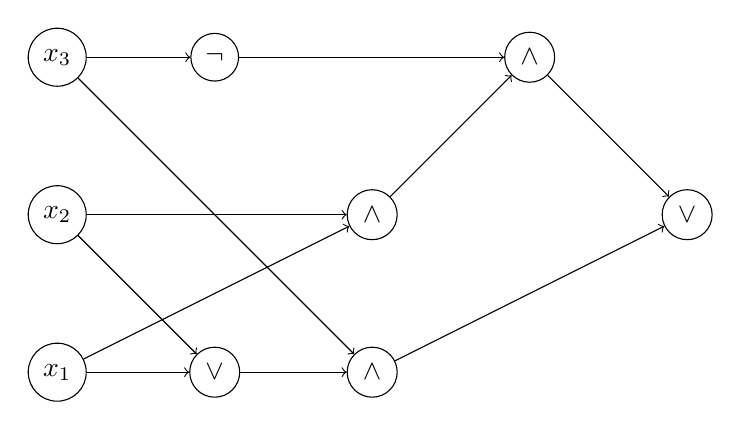
\begin{tikzpicture}[scale=1, transform shape]
        \tikzstyle{every node}=[circle,draw, minimum size=0.5cm]
        \node (s1)  at (0,0) {$ x_1 $};
        \node (s2)  at (0,2) {$ x_2 $};
        \node (s3)  at (0,4) {$ x_3 $};

        \node (s4)  at (2,0) {$ \vee $};
        \node (s5)  at (2,4) {$ \neg $};

        \node (s6)  at (4,0) {$ \wedge $};
        \node (s7)  at (4,2) {$ \wedge $};

        \node (s8)  at (6,4) {$ \wedge $};

        \node (s9)  at (8,2) {$ \vee $};

        \path [->] (s1) edge  (s4);
        \path [->] (s2) edge  (s4);
        \path [->] (s3) edge  (s5);

        \path [->] (s4) edge  (s6);
        \path [->] (s3) edge  (s6);
        \path [->] (s1) edge  (s7);
        \path [->] (s2) edge  (s7);

        \path [->] (s5) edge  (s8);
        \path [->] (s7) edge  (s8);

        \path [->] (s6) edge  (s9);
        \path [->] (s8) edge  (s9);
    \end{tikzpicture}
    \caption{Пример булевой схемы в стандартном базисе.}
    \label{fig:boolean:scheme_example}
\end{figure}

\begin{Answer}
    \noindent
    Идя от последнего присваивания вниз к переменным, выписываем формулу.
    Если какая-то вершина уже встречалось ранее в правой части присваивания,
    <<копируем>> соответствующую часть формулы.
    \[
        f(x_1, x_2, x_3) = \left[ (x_1 \vee x_2) \wedge x_3 \right] \vee \left[ (x_1 \wedge x_2) \wedge \neg x_3 \right]
    \]
    Можно заметить, что переиспользований не было;
    данная булева изначально ялвяется формулой.
    В качестве упражнения роверьте справедливость утверждения \ref{statement:boolean:schemes_to_graphs}.
\end{Answer}


\begin{Exercise}[counter=SecExercise, label={exercise:boolean:f_existance}]
    \noindent
    Существует ли такая булева функция $ f $ от двух переменных,
    что схема в базисе $ \{\wedge, f \} $
    \[
        x_1, \; x_2, \; s_3 = f(x_1, x_2), \; s_4 = f(x_2, x_1), \; s_5 = s_3 \wedge s_4
    \]
    вычисляет \textbf{а)} функцию $ x_1 $? \textbf{б)} функцию $ x_1 \oplus x_2 $?
\end{Exercise}

\begin{Answer}
    \noindent
    \begin{enumerate}[label=\textbf{\alph*)}]
        \item
            Заметим, что схема симметрична относительно перестановки $ x_1 $ и $ x_2 $.
            Из этого следует, что вычисляемая функция также должна быть симметрична относительно перестановки аргументов местами.
            Но для функции $ x_1 $ это неверно.
            Значит, ответ~--- нет.
        \item
            Да, $ f(x_1, x_2) = x_1 \oplus x_2 $.
            Тогда схема эквивалентна формуле
            \[
                f(x_1, x_2) \wedge f(x_2, x_1) = (x_1 \oplus x_2) \wedge (x_2 \oplus x_1) = x_1 \oplus x_2
            \]
    \end{enumerate}
\end{Answer}


\begin{Exercise}[counter=SecExercise, label={exercise:boolean:move_negation_to_arguments}]
    \noindent
    Докажите, что всякую булеву схему в стандартном базисе размера $ m $ с $ n $ переменными можно переделать в булеву схему размера не более $ 2 \cdot m $,
    вычисляющую ту же формулу, и в которой все отрицания применяются только к переменными.
\end{Exercise}

\begin{Answer}
    \noindent
    Приведём явный алгоритм данного преобразования.
    Для каждой схемы введём $ q $~--- суммарное число связок $ \vee $ и $ \wedge $,
    $ p $~--- число связок $ \neg $,
    а также $ k $~--- такое число,
    что все присваивания начиная с $ (k + 1) $-го гарантированно не являются отрицаниями.
    Изначально $ k $ положим равным $ m $, так как последнее присваивание может быть отрицанием.
    Также введём число $ d $, равное числу связок $ \vee $ и $ \wedge $, имеющих номер, не больший $ k $.

    Алгоритм построен так, что $ d $ и $ k $ не увеличиваются, $ q $ не меняется.
    Непосредственно описание алгоритма приведено ниже:
    \begin{enumerate}
        \item $ k \leftarrow m $, $ d \leftarrow q = m - n - p $.
        \item
            Если $ d = 0 $, то нет ни одного отрицания, применяемого к конъюнкции или дизъюнкции.
            Тогда алгоритм завершается.

            В противном случае рассмотрим $ k $-ое присвоение.
            Имеем следующие варианты, чем оно является:
            \begin{enumerate}
                \item[$ x_i $]
                    Реализация данного случая возможна,
                    только если в схеме не осталось отрицаний.
                    Таким образом, алгоритм завершается.
                \item[$ \vee $, $ \wedge $]
                    Данное присвоение не является результатом отрицания.
                    Можем уменьшить $ k $ и $ d $ на единицу.
                    Схему оставляем неизменной.
                \item[$ \neg $]
                    Рассмотрим, к чему применяется отрицание.
                    Имеем следующие варианты:
                    \begin{enumerate}
                        \item[$ \neg $]
                            Пользуясь тождеством $ \neg \neg x $, убираем два отрицания.
                            Числа $ p $ и $ k $ уменьшаются на два,
                            число остальных связок не меняется;
                            $ d $ также неизменно.
                        \item[$ \vee $, $ \wedge $]
                            Пользуясь законами де Моргана,
                            вносим отрицание в аргументы связки;
                            тем самым $ p $ увеличивается на единицу, $ k $ не меняется, $ d $ уменьшается на единицу.
                            Поскольку обязательно $ d \geqslant 0 $,
                            данный пункт реализуется не более $ q = const $ раз.
                        \item[$ x_i $]
                            Рассматриваемое отрицание уже применяется к переменной.
                            Изменим нумерацию в схеме так, чтобы выбранное отрицание стояло до любой из связок $ \vee $ или $ \wedge $
                            (если это уже так, ничего делать не надо).
                            Данный пункт реализуется не более $ m $ раз,
                            поскольку число таких отрицаний не превышает $ k \leqslant m $,
                            и каждое из них рассматривается единожды.
                    \end{enumerate}
            \end{enumerate}
        \item
            Перейти к предыдущему пункту.
    \end{enumerate}

    Алгоритм завершит свою работу, так как $ k $ не может быть отрицательным,
    а на каждом шаге оно не увеличивается;
    при этом число шагов, на которых $ k $ оставалось неизменным, ограничено.

    В ходе работы алгоритма $ q $ оставалось неизменным,
    а $ p $ либо уменьшалось на $ 2 $ за какие-то шаги,
    либо увеличивалось на $ 1 $ за шаги, когда $ k $-ое присвоение являлось отрицанием конъюнкции или дизъюнкции;
    второй вариант реализовался не более $ m $ раз.
    Таким образом, размер схемы увеличится не более, чем в два раза.
\end{Answer}



\subsection{Классы булевых функций}
\label{subsec:boolean:boolean_functions_classes}

В прошлом разделе мы ввели понятие булевой схемы, заданной некоторым базисом.
Связь описательной способности булевых схем с базисом очевидна:
если базис слишком <<беден>> (например, состоит из одного только отрицания),
далеко не все булевы функции представимы в виде схемы в выбранном базисе.
В данном разделе эта связь будет исследована полее подробно и формально.
Начнём с определений.


\begin{definition}
    \label{definition:boolean:all_boolean_functions}
    Определим\footnote{Это исключительно авторское обозначение. Не рекомендуется использовать без определения.}
    \defemph{множество всех булевых функций} от конечного числа переменных:
    $ \boolfun \defeq \bigcup_{k=0}^\infty \{0, 1\}^k \times \{0, 1\} $.
\end{definition}


\begin{definition}
    \label{definition:boolean:closure}
    \defemph{Замыканием} $ \closure (B) $ некоторого базиса $ B \subseteq \boolfun $ будем называть множество булевых функций,
    представимых в виде схемы в данном базисе.
    \\[0.25\baselineskip]
    Множество $ B $ булевых функций называется \defemph{замкнутым} в случае $ B = \closure (B) $.
\end{definition}


\begin{statement}
    \label{statement:boolean:closure_is_closed}
    Замыкание любого множества функций замкнуто.
    Иначе говоря, $ \forall B \subseteq \boolfun \;\, \closure(B) = \closure(\closure(B)) $.
\end{statement}


\begin{definition}
    \label{definition:boolean:complete_class}
    Множество $ B $ булевых функций называется \defemph{полным} в случае $ \closure (B) = \boolfun $.
\end{definition}


Оказывается, один полный базис нам уже известен.
Это стандартный базис.
Для того, чтобы доказать его полноту, введём несколько впомогательных определений.

\begin{definition}
    \label{definition:boolean:literal}
    \defemph{Литералом} называют переменную или отрицание переменной.
    Введём следующие обозначения для литералов: $ x^0 = \neg x $, $ x^1 = x $.
\end{definition}

\begin{definition}
    \label{definition:boolean:clause}
    \defemph{Конъюнктом} и \defemph{дизъюнктом} называют конъюнкцию и дизъюнкцию литералов соответственно:
    \[
        C = l_1 \wedge l_2 \wedge \ldots \wedge l_n, \qquad D = l_1 \vee l_2 \vee \ldots \vee l_m
    \]
\end{definition}


\begin{remark}
    \label{remark:boolean:clause_true_false}
    Конъюнкт $ x_1^{\alpha_1} \wedge x_2^{\alpha_2} \wedge \ldots \wedge x_n^{\alpha_n} $ принимает истинное значение только на наборе $ x_i = \alpha_i $.
    Дизъюнкт $ x_1^{\alpha_1} \vee x_2^{\alpha_2} \vee \ldots \vee x_m^{\alpha_m} $ принимает ложное значение только на наборе $ x_i = \neg \alpha_i $.
\end{remark}


\begin{definition}
    \label{definition:DNF_CNF}
    Формулы вида
    \[
        \bigvee_{(\alpha_1, \ldots, \alpha_n) \in \mathcal{A}} x_1^{\alpha_1} \wedge x_2^{\alpha_2} \wedge \ldots \wedge x_n^{\alpha_n}
        \qquad
        \bigwedge_{(\alpha_1, \ldots, \alpha_n) \in \mathcal{A}} x_1^{\alpha_1} \vee x_2^{\alpha_2} \vee \ldots \vee x_n^{\alpha_n}
    \]
    называются \defemph{дизъюнктивной} и \defemph{конъюнктивной нормальными формами} соответственно.
    Здесь $ \mathcal{A} \subseteq \{0, 1\}^n $.
\end{definition}


\begin{theorem}
    \label{theorem:boolean:standard_basis_complete}
    Стандартный базис является полным, то есть $ \closure(\{\vee, \wedge, \neg\}) = \boolfun $.
\end{theorem}

\begin{proof}
    Пусть имеется произвольная булева функция $ f: \{0, 1\}^n \rightarrow \{0, 1\} $.
    Заметим, что
    \[
        f(x_1, \ldots, x_n) = \bigvee_{(\alpha_1, \ldots, \alpha_n) \in f^{-1}(1)} x_1^{\alpha_1} \wedge x_2^{\alpha_2} \wedge \ldots \wedge x_n^{\alpha_n}
    \]
    Действительно, согласно замечанию \ref{remark:boolean:clause_true_false},
    каждый конъюнкт принимает истинное значение только на одном наборе значений переменных.
    По построению этот набор является выполняющим набором для функции $ f $.
    Также из определения полного прообраза $ f^{-1}(1) $ следует, что все подобные наборы были рассмотрены.
\end{proof}

Для доказательства было использовано разложение в ДНФ.
Точно также можно было бы представить функцию и в виде КНФ.

\begin{Exercise}[counter=SecExercise, label={exercise:boolean:DNF_example}]
    \noindent
    Разложите в ДНФ и КНФ булеву функцию, заданную вектором
    значений: $ f(x_1, x_2, x_3) = 10100101 $.
\end{Exercise}

\begin{Answer}
    \noindent
    Облегчим себе жизнь, заметив, что $ x_2 $~--- фиктивная переменная.
    Пользуясь алгоритмом из теоремы \ref{theorem:boolean:standard_basis_complete},
    \[
        f(x_1, x_2, x_3) = (\neg x_1 \wedge \neg x_3) \vee (x_1 \wedge x_3) = (\neg x_1 \vee x_2) \wedge (x_1 \vee \neg x_2)
    \]
\end{Answer}


\begin{corollary}
    \label{corollary:boolean:substandard_basis_complete}
    Базисы $ \{ \vee, \neg \} $ и $ \{ \wedge, \neg \} $ полны.
\end{corollary}

\begin{proof}
    Следует из законов де Моргана и полноты стандартного базиса
\end{proof}


\begin{corollary}
    \label{corollary:boolean:Zhegalkin_basis_complete}
    Базис $ \{ 1, \oplus, \wedge \} $ полон.
\end{corollary}

\begin{proof}
    Аналогично, используя $ \neg x = 1 \oplus x $.
\end{proof}


\begin{definition}
    \label{definition:boolean:Zhegalkin_polynomials}
    Формулы, заданные в базисе $ \{1, \oplus, \wedge \} $, называются \defemph{полиномами Жегалкина}.
\end{definition}

Следствия выше демонстрируют один из способов доказательства полноты базиса, а именно сведение к стандартному базису.
Однако открытым остаётся вопрос, как доказывать неполноту.
Оказывется, для этого есть специальная теорема.
Прежде чем к ней перейти, определим так называемые \defemph{классы Поста}:

\begin{definition}
    \label{definition:boolean:Post_classes}
    \defemph{Классами Поста} называются следующие пять множеств булевых функций:
    \begin{enumerate}
        \item[($ M $)] \defemph{Монотонные функции}:
            \[
                M = \{ f \in \boolfun \mid \forall x_1, x_2 \in \{0, 1\}^n \;\, (x_1 \leqslant x_2) \rightarrow (f(x_1) \leqslant f(x_2)) \},
            \]
            где порядок на $ \{0, 1\}^n $ берётся покоординатный.
        \item[($ L $)] \defemph{Линейные функции}: $ L = \closure(\{1, \oplus\}) $.
        \item[($ T_0 $)] \defemph{Функции, сохраняющие ноль}: $ T_0 = \{ f \in \boolfun \mid f(0, \ldots, 0) = 0 \} $.
        \item[($ T_1 $)] \defemph{Функции, сохраняющие единицу}: $ T_1 = \{ f \in \boolfun \mid f(1, \ldots, 1) = 1 \} $.
        \item[($ S $)] \defemph{Самодвойственные функции}: $ M = \left\{ f \in \boolfun \mid \neg f(\neg x_1, \ldots, \neg x_n) = f(x_1, \ldots, x_n) \right\} $
    \end{enumerate}
\end{definition}

\begin{theorem}[Поста]
    \label{theorem:boolean:Post}
    Замкнутое множество булевых функций является неполным тогда и только тогда, когда содержится в одном из классов Поста.
\end{theorem}


\begin{Exercise}[counter=SecExercise, label={exercise:boolean:preserves_0_1}]
    \noindent
    Сколько имеется булевых функций от $ n $ переменных,
    сохраняющих одновременно <<$ 0 $>> и <<$ 1 $>>?
\end{Exercise}

\begin{Answer}
    \noindent
    Условие сохранения <<$ 0 $>> и <<$ 1 $>> <<блокирует>> первую и последнюю из $ 2^n $ строк в таблице истинности;
    на остальных же наборах переменных данные функции могут принимать произвольные значения.
    Тогда ответ~--- $ 2^{2^n - 2} $.
\end{Answer}


\begin{Exercise}[counter=SecExercise, label={exercise:boolean:Post_example}]
    \noindent
    Являются ли полными следующие базисы?
    При отрицательном ответе укажите, в каких из классов $ T_0 $, $ T_1 $, $ M $, $ L $, $ S $ лежит замыкание базиса.
    \begin{enumerate}[label=\textbf{\alph*)}]
        \item $ \{ \neg, \rightarrow \} $, где $ \rightarrow $~--- импликация;
        \item $ \{ \downarrow \} $, где $ x \downarrow y $ равна $ \neg x \wedge \neg y $ (стрелка Пирса);
        \item $ \{ \wedge, \vee, \setminus \} $, где $ x \setminus y $ равна $ x \wedge \neg y $;
        \item $ \{ 1, \oplus \} $;
        \item $ \{ \neg, \leftrightarrow \} $, где $ x \leftrightarrow y $ равна $ (x \rightarrow y) \wedge (y \rightarrow x) $.
    \end{enumerate}
\end{Exercise}

\begin{Answer}
    \noindent
    \begin{enumerate}[label=\textbf{\alph*)}]
        \item
            Базис полный, так как $ \neg x \rightarrow y = x \vee y $,
            а потому $ \closure(\{\neg, \rightarrow\}) = \closure(\{\neg, \vee\}) = \boolfun $.
        \item
            Базис полный, так как $ x \downarrow x = \neg x $,
            $ \neg x \downarrow \neg y = x \wedge y $,
            а потому $ \closure(\{ \downarrow \}) = \closure(\{\neg, \downarrow\}) = \closure(\{\neg, \wedge\}) = \boolfun $.
        \item
            Нет, данный базис неполный: все функции сохраняют ноль.
            При этом $ \wedge \notin L, S $; $ \setminus \notin T_1, M $.
            Таким образом, базис целиком лежит только в одном классе: $ \{\wedge, \vee, \setminus \} \subseteq T_0 $.
        \item
            Нет, данный базис неполный: все функции линейны.
            При этом $ 1 \notin T_0, S $; $ \oplus \notin M, T_1 $.
        \item
            Нет, данный базис неполный: все функции линейны: $ \neg x = 1 \oplus x $, $ x \leftrightarrow y = 1 \oplus x \oplus y $.
            При этом $ \neg \notin T_0, T_1 $; $ \leftrightarrow \notin S, M $.
    \end{enumerate}
\end{Answer}


\begin{Exercise}[counter=SecExercise, label={exercise:boolean:linear_closure}]
    \noindent
    Постройте замыкание базиса $ \{\neg, \oplus\} $.
\end{Exercise}

\begin{Answer}
    \noindent
    Заметим, что $ 1 = \neg (x \oplus x) $ и $ \neg x = 1 \oplus x $.
    Отсюда следует, что $ \closure(\{\neg, \oplus\}) \subseteq \closure(\{1, \oplus\}) $ и $ \closure(\{1, \oplus\}) \subseteq \closure(\{\neg, \oplus\}) $.
    Значит, $ \closure(\{\neg, \oplus\}) = \closure(\{1, \oplus\}) = L $.
\end{Answer}

\begin{Exercise}[counter=SecExercise, label={exercise:boolean:monotonous_and_MAJ}]
    \noindent
    Назовём функцией большинства $ \text{MAJ}(x_1, x_2,\ldots , x_n) $ булеву функцию,
    значение которой совпадает с тем значением,
    которое принимает большинство переменных (если мнения разделились поровну, $ \text{MAJ} = 0 $).
    Схемы в базисе $ \{\vee, \wedge, 1, 0 \} $ называются монотонными.
    Вычисляется ли $ \text{MAJ} $ монотонной схемой?
\end{Exercise}

\begin{Answer}
    \noindent
    Да, вычисляется.
    Заметим, что
    \[
        \text{MAJ}(x_1, \ldots, x_n) = \bigvee_{I \in \binom{\{1, \ldots, m\}}{\lfloor n/2 \rfloor + 1}} \bigwedge_{i \in I} x_i
    \]
    Действительно, любой набор значений $ x_1, \ldots, x_n $, в котором единиц большинство, выполняет хотя бы один конъюнкт справа.
    Также любой набор значений входных переменных, выполняющий правую формулу, содержит более $ n/2 $ единиц,
    из чего следует выполнение на нём же и $ \text{MAJ} $.
    Таким образом, получена ДНФ без отрицаний, что и требовалось по условию.
\end{Answer}


\begin{Exercise}[counter=SecExercise, label={exercise:boolean:self_dual}]
    \noindent
    \begin{enumerate}[label=\textbf{\alph*)}]
        \item
            Являются ли самодвойственными функции $ x_1 \vee x_2 $, $ x_1 \wedge x_2 $?
        \item
            Докажите, что схема в базисе, состоящем из самодвойственных функций,
            вычисляет самодвойственную функцию.
    \end{enumerate}
\end{Exercise}

\begin{Answer}
    \noindent
    \begin{enumerate}[label=\textbf{\alph*)}]
        \item
            Нет: $ \neg(\neg x_1 \vee \neg x_2) = x_1 \wedge x_2 \neq x_1 \vee x_2 $.
        \item
            Эквивалентное определение самодвойственности:
            \[
                \neg f(x_1, \ldots, x_n) = f(\neg x_1, \ldots, \neg x_n)
            \]
            Для начала перейдём от схемы к формуле.
            Далее рассмотрим отрицание формулы и согласно эквивалентному определению самодвойственности будем <<спускать>> отрицания до тех пор,
            пока не дойдём до аргументов.
            Получим, что отрицание формулы равно формуле от отрицаний аргументов.
            Это эквивалентно самодвойственности.
    \end{enumerate}
\end{Answer}


\begin{Exercise}[counter=SecExercise, label={exercise:boolean:not_self_dual}]
    \noindent
    Пусть $ f(x_1, \ldots, x_n) $~--- несамодвойственная функция.
    Докажите, что константы $ 0 $, $ 1 $ вычисляются в базисе $ \{\neg, f \} $.
\end{Exercise}

\begin{Answer}
    \noindent
    Раз $ f $ не самодвойственная,
    $ \exists x_1, \ldots x_n: \neg f(\neg x_1, \ldots, \neg x_n) \neq f(x_1, \ldots, x_n) $.
    Обозначим любой их таких наборов значений как $ \{ \alpha_i \} $.
    Тогда заметим, что $ f(x^{\alpha_1}, \ldots, x^{\alpha_n}) = const $.
    Действительно, если это не так, то либо $ f(x^{\alpha_1}, \ldots, x^{\alpha_n}) = x $,
    либо $ f(x^{\alpha_1}, \ldots, x^{\alpha_n}) = \neg x $
    (других булевых функций одной переменной нет).
    Но $ f_1(x) = x $ и $ f_2(x) = \neg x $ самодвойственны.
    Тогда $ f(1^{\alpha_1}, \ldots, 1^{\alpha_n}) = \neg f(0^{\alpha_1}, \ldots, 0^{\alpha_n}) $
    что противоречит выбору $ \alpha_i $.
    Значит $ f(x^{\alpha_1}, \ldots, x^{\alpha_n}) = const $,
    а другую константу можно получить, взяв отрицание.
\end{Answer}
